\section{Επεξεργασία Δεδομένων}

\begin{frame}{Δεδομένα}
	
	Σε κάθε γεγονός είναι δεδομένα τα εξής:
	%
	\vspace{4mm}
	%
	\begin{itemize}
		\item Αριθμός \dvtrue.
		\item Η θέση κάθε \dvtrue.
		\item Αριθμός τροχιών.
		\item Το πρώτο σημείο $\mathrm{P_i}$ και το τελευταίο σημείο $\mathrm{P'_i}$ της $i$-οστής τροχιάς.
	\end{itemize}
\end{frame}

\beamerdefaultoverlayspecification{}

\begin{frame}{Διαδικασία Επεξεργασίας}
	
	\begin{columns}
	%
	\column{0.55\textwidth}
		\begin{enumerate}
		\item \textbf{Απόσταση Mεταξύ Eυθειών}
			
			\begin{equation*}
				\vb{\mathrm{OA}} = \vb{r}_\mathrm{i} + \frac{\vb{u}\vdot(\vb{n}_\mathrm{j}\cross\vb{r}_\mathrm{o})}{\norm{\vb{u}}^2}\,\vb{n}_\mathrm{i}, \quad
			\end{equation*}
			%
			\begin{equation*}
				\vb{\mathrm{OB}} = \vb{r}_\mathrm{j} + \frac{\vb{u}\vdot(\vb{n}_\mathrm{i}\cross\vb{r}_\mathrm{o})}{\norm{\vb{u}}^2}\,\vb{n}_\mathrm{j}, \quad
			\end{equation*}
			%
			\vspace{0.05cm}
			%
			\begin{equation*}
				\vb{n}_\mathrm{i} \equiv \vb{r}'_\mathrm{i} - \vb{r}_\mathrm{i}, \ \vb{n}_\mathrm{j} \equiv \vb{r}'_\mathrm{j} - \vb{r}_\mathrm{j}.
			\end{equation*}
			%
			\begin{equation*}
				\vb{u} \equiv \vb{n}_\mathrm{j}\cross\vb{n}_\mathrm{i}, \ \vb{r}_\mathrm{o} \equiv \vb{r}_\mathrm{j} - \vb{r}_\mathrm{i},
			\end{equation*}
			%
			\seti
		\end{enumerate}
	%
	\column{0.45\textwidth}	
		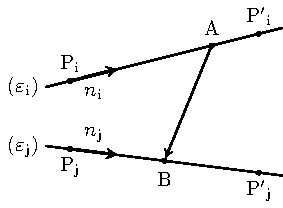
\includegraphics{line_distance}
	\end{columns}
\end{frame}

\begin{frame}{Διαδικασία Επεξεργασίας}
	
	\begin{columns}
	\column{0.6\textwidth}	
	\begin{enumerate}
		\conti
		\item \textbf{Συνθήκες Επιλογής \dvrecobf}
		\seti
	\end{enumerate}
	\vspace{4 mm}
	\begin{itemize}%[<+->]
		\item Κάθε \dvreco\,: 
			\begin{itemize}
				\item ανακατασκευάζεται από δύο τροχιές, και
				\item είναι το μέσο του διανύσματος απόστασής τους.
			\end{itemize}
		\item Οι γωνίες: $0\leq\theta_\mathrm{i},\, \theta_\mathrm{j} \leq \pi/2$.
		\item Η απόσταση τροχιών μικρό- τερη ή ίση του \texttt{DVCut = 11}.
	\end{itemize}
	%
	\column{0.4\textwidth}
	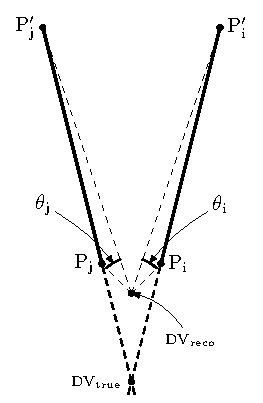
\includegraphics{Lines-DV}
	\end{columns}
\end{frame}

\begin{frame}{Διαδικασία Επεξεργασίας}
	
	\begin{columns}
	\column{0.7\textwidth}
	\begin{enumerate}
		\conti
		\item \textbf{Πολλαπλές Τροχιές που Ανήκουν σε }\dvrecobf
		\seti
	\end{enumerate}
	%
	\begin{itemize}
		\item Έλεγχος για τροχιές που δεν έχουν χρησιμοποιηθεί για ανακατασκευή \dvreco.
		\item Η απόστασή τους:
			\begin{equation*}
				d_\mathrm{i} = \frac{\norm{(\vb{p}-\vb{r}_\mathrm{i})\cross\vb{n}_\mathrm{i})}}{\norm{\vb{n}_\mathrm{i}}},\ \vb{n}_\mathrm{i} \equiv \vb{r}'_\mathrm{i}-\vb{r}_\mathrm{i}
			\end{equation*}
		 από το \dvreco\ μικρότερη από \texttt{TrajectoryCut}.
	\end{itemize}
	%
	\column{0.3\textwidth}	
	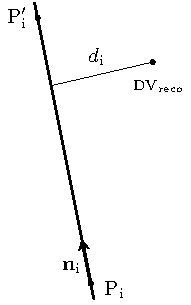
\includegraphics{line-to-point-distance}
	\end{columns}
\end{frame}

\beamerdefaultoverlayspecification{<+->}

\begin{frame}{Διαδικασία Επεξεργασίας}
	
	\begin{enumerate}
		\conti
		\item \textbf{Τροχιές που Έχουν Χρησιμοποιηθεί}
		\seti
	\end{enumerate}
	%
	\vspace{4 mm}
	%
	\begin{itemize}
		\item Σε κάθε τροχιά αντιστοιχίζεται ένας δείκτης.
		\item Στον πίνακα \texttt{usedLineIndex} αποθηκεύονται οι δείκτες από τις τροχιές που έχουν χρησιμοποιηθεί:
			\begin{itemize}
				\item Είτε για την ανακατασκευή κάποιου \dvreco,
				\item είτε γιατί ανήκουν σε κάποιο \dvreco.
			\end{itemize}
	\end{itemize}	
\end{frame}

\begin{frame}{Διαδικασία Επεξεργασίας}
	
	\begin{enumerate}
		\conti
		\item \textbf{Υπολογισμός Σφαλμάτων}
		\seti
	\end{enumerate}
	%
	\vspace{4 mm}
	%
	Για κάθε \dvreco\ που υπολογίζεται ακολουθείται η εξής διαδικασία:
	\begin{itemize}
		\item Υπολογίζονται όλα τα σφάλματα με τα \dvtrue\ που υπάρχουν στο γεγονός.
		\item Το σφάλμα που αντιστοιχεί στο εκάστοτε \dvreco\ είναι το μικρότερο από τα παραπάνω.
	\end{itemize}
\end{frame}